% Include from the paperfuture repository root; requires \usepackage{graphicx}.
\begin{figure*}[t]
  \centering
  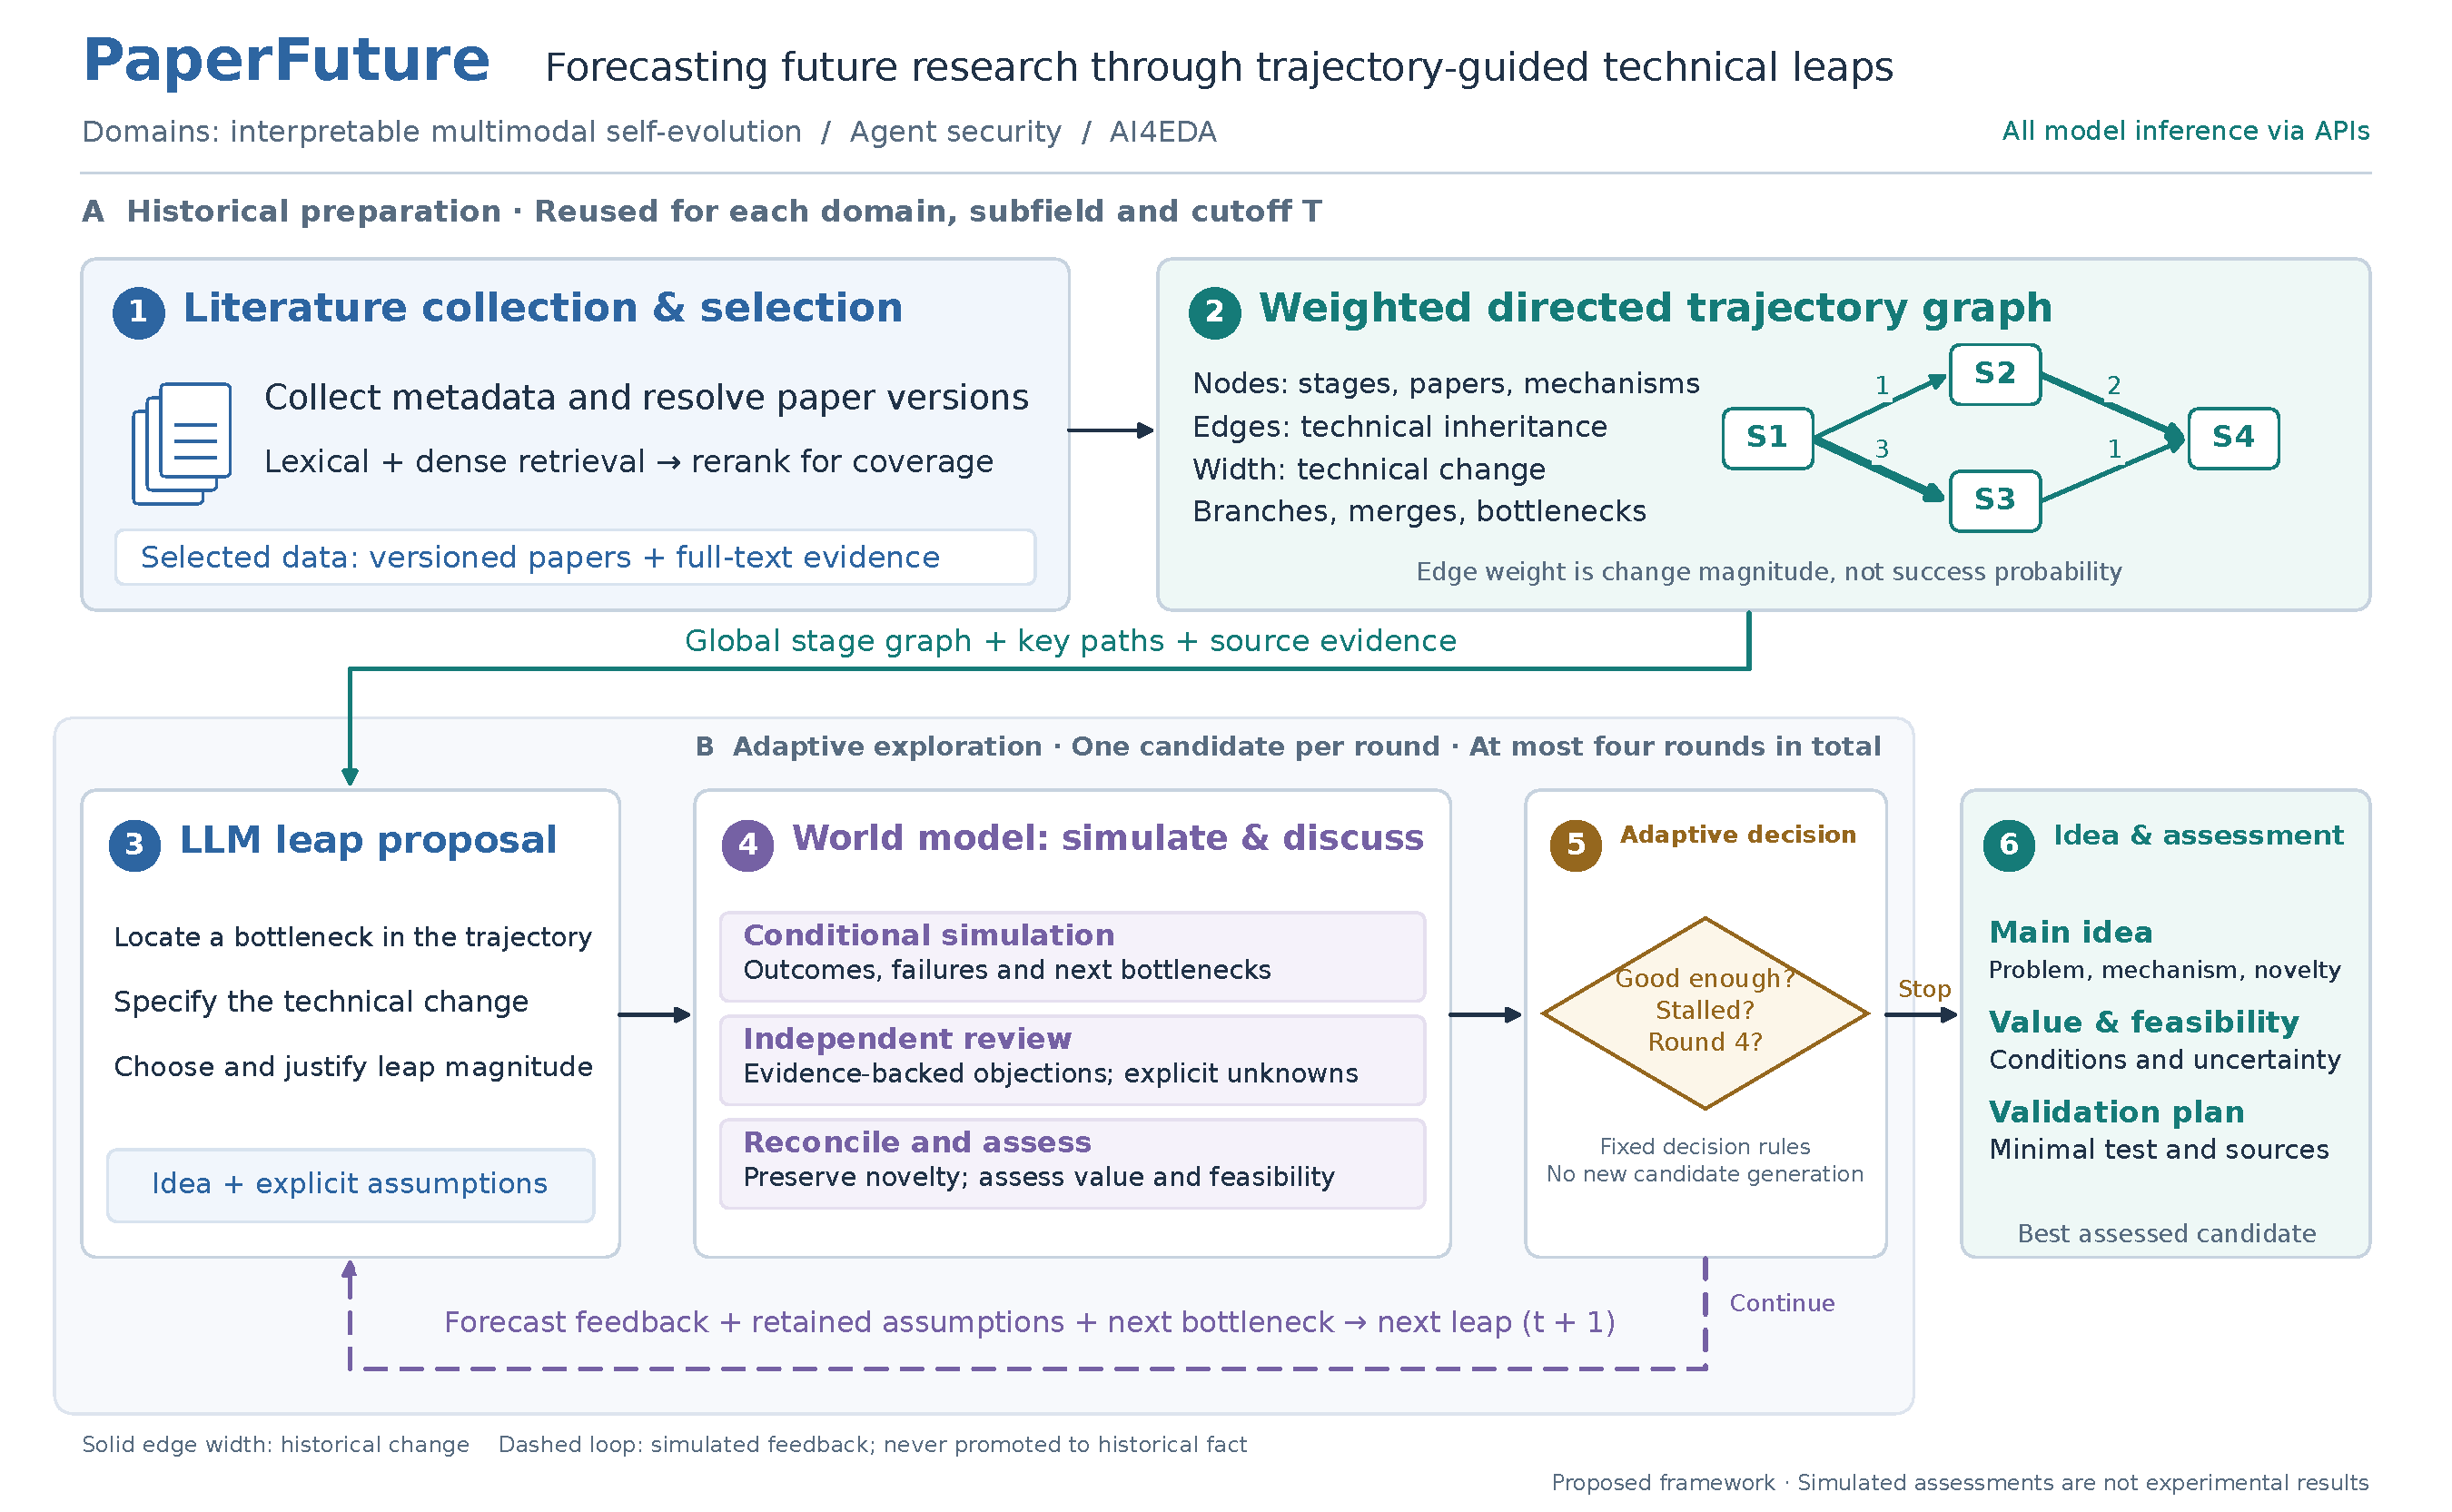
\includegraphics[width=\textwidth]{figures/paperfuture_framework_en.pdf}
  \caption{Proposed PaperFuture framework.
  (1--2) Versioned literature is selected for relevance and trajectory coverage,
  then organized into a directed graph of research stages with evidence-backed
  technical transitions. Edge width encodes the magnitude of technical change.
  (3--5) An LLM proposes a leap using the global stage graph and detailed evidence.
  A research world model simulates conditional outcomes, reviews objections and
  assesses value and feasibility. Fixed decision rules either stop exploration
  or return the predicted bottlenecks and retained assumptions to the next leap.
  All candidates share a global limit of four exploration rounds.
  (6) The best assessed candidate is returned with its value, feasibility,
  uncertainty and validation plan. Dashed arrows carry simulated feedback;
  these predictions are never promoted to facts in the historical graph.
  All model inference uses APIs. This figure specifies the intended system;
  it does not claim completed implementation or validated forecasting performance.}
  \label{fig:paperfuture-framework}
\end{figure*}
